\chapter{Methodology}
\label{sec:methodology}
In this chapter, an overview of the concepts, algorithms and machine learning models encountered throughout this thesis work is provided.

\section{Optimization problems}
\label{sec:opt_prob}
Everything in machine learning comes down to an optimization problem.

Optimization is the problem of finding one or more points that minimize or maximize a given objective function.

\begin{definition}[Optimization problem]
Let $J:A \subseteq \mathbb{R}^n \to \mathbb{R}$. The problem of finding a global minimizer $\mathbf{x^*} \in B \subseteq A$ of $J$ is an called optimization problem.
\end{definition}
$B$ is called the \textit{search space}. When $A=B$, the optimization problem is \textit{unconstrained}, whereas if $A \subset B$ it is \textit{constrained}; in constrained optimization problems typically $B$ is defined by a set of constraints, i.e. equalities and/or inequalities that points in $B$ have to satisfy. Points in $B$ are called \textit{feasible solutions}, whereas all the possible $\mathbf{x^*}$ (if existent) are called \textit{optimal solutions}.

There are a number of results which guarantee the existence and uniqueness of the optimal solution(s) of an optimization problem.

\begin{definition}[Convex set]
A set $C \subseteq \mathbb{R}^n$ is convex if $\forall \mathbf{x},\mathbf{y} \in C$ the segment joining $\mathbf{x}$ and $\mathbf{y}$ is contained in $C$:
\[
\alpha \mathbf{x} + (1-\alpha)\mathbf{y} \in C \qquad \forall \alpha \in (0,1)
\]
\end{definition}

\begin{definition}[Convex function]
Given a convex set $C \subset \mathbb{R}^n$, a function $f:C \to \mathbb{R}$ is convex if
\[
f(\alpha \mathbf{x}+(1-\alpha)\mathbf{y}) \leq \alpha f(\mathbf{x}) + (1-\alpha) f(\mathbf{y}) \qquad \forall \mathbf{x},\mathbf{y} \in C, \; \alpha \in (0,1)
\]
\end{definition}
If the inequality in the definition holds strictly, then the function is strictly convex.

\begin{theorem}
If $f$ is convex on $B$, local minimizers of $f$ in $B$ are also global minimizers. Moreover, if $f$ is also strictly convex on $B$, then there exist a unique global minimizer of $f$ in $B$.
\end{theorem}

An optimization problem is (strictly) convex if $J$ is a (strictly) convex function. In machine learning, the objective function $J$ is usually a continuous non-linear function, and it is commonly called \textit{cost function}.

Direct methods for solving non-linear optimization problems are often too impractical. Luckily, there exist a huge number of \textbf{iterative methods} for solving optimization problems, i.e. methods which construct a sequence $\mathbf{x}_0,\mathbf{x}_1,\dots$ which are asymptotically likely to converge to the optimal solution. Three of them are discussed hereafter: gradient descent (sec. \ref{sec:gradient_descent}), stochastic gradient descent (sec. \ref{sec:sgd}), Nelder-Mead method (sec. \ref{sec:nelder_mead}).



\subsection{Gradient descent}
\label{sec:gradient_descent}
\textbf{Gradient descent} \cite{gd} is an iterative method in which the iterates $\mathbf{x}_k$ are obtained by moving along the local direction of steepest descent, i.e. $-\nabla J(\mathbf{x}_k)$:
\begin{equation}
\mathbf{x}_{k+1} = \mathbf{x}_k - \eta \nabla J(\mathbf{x}_k)
\end{equation}
Basically, at each step the gradient descent algorithm locally builds a first-order approximation of $J$ at $\mathbf{x}_k$, and then moves along the local direction of most rapid decrease of $J$ (which is minus the gradient of $J$ at $\mathbf{x}_k$) until a stopping criterion is met (e.g. threshold on $\norm{J(\mathbf{x}_{k+1}) - J(\mathbf{x}_k)}$ reached and/or maximum number of iterations reached; both are user-specified hyperparameters).

In machine learning, the step-length $\eta \in \mathbb{R}$ is commonly known as \textit{learning rate}. It is a user-defined hyperparameter which must be chosen carefully: a learning rate which is too high may make the method fail to converge, whereas a learning rate which is too low may slow down convergence. This is exemplified in fig. \ref{fig:lr_choice}.

\begin{figure}[hbt!]
    \centering
    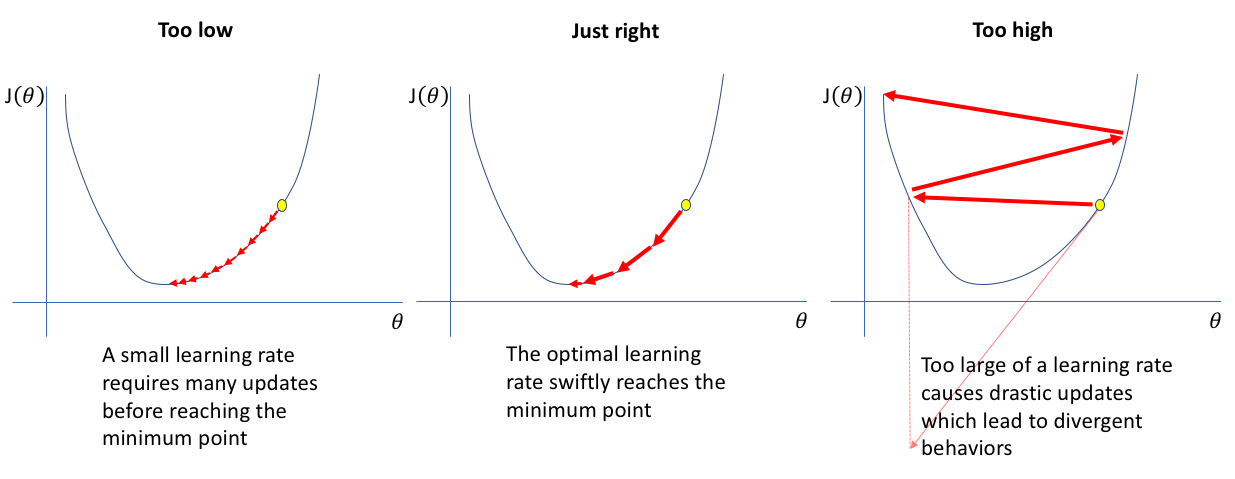
\includegraphics[width=\textwidth]{images/lr_choice}
    \caption[Choice of the learning rate of gradient descent]{The importance of choosing an appropriate learning rate for the gradient descent algorithm. Taken from \cite{lr_choice}}
    \label{fig:lr_choice}
\end{figure}

Typically, when the method is approaching the minimum of the function that is being optimized, we may want to decrease the learning rate to allow more fine-grained updates. There exists a huge variety of rules and schedules for the update of the learning rate \cite{lr_schedules}. Among them:
\begin{itemize}
    \item Reduce $\eta$ by a factor $\xi \in (0,1)$ when $\norm{J(\mathbf{x}_{k+1}) - J(\mathbf{x}_k)}$ is below a specified threshold $T$ for at least $P$ iterations. $\xi$ (learning rate decay factor), $T$ (tolerance) and $P$ (patience) are all user-specified hyperparameters (and they can be scheduled as well!). Typically implemented when training neural networks (sec. \ref{sec:neural_network}).
    \item Reduce $\eta$ at each step by a factor $g(k)$ where $g$ is a decreasing function of $k$ (e.g. $g(k) = \frac{1}{k^p}$, with $p>0$ hyperparameter). $g$ is a user-specified hyperparameter. Used by default in scikit-learn when training ridge regression (sec. \ref{sec:ridge}) via SGD.
\end{itemize}

Also the choice of the initial point $\mathbf{x}_0$ is of particular importance: choosing it to be near the effective minimum of the function may speed up the convergence of the method. However, quite obviously, this information is almost never available, and we must resort to random initialization.

\smallskip

Since non-linear functions are not convex in general, they may have many local minima, as shown in fig. \ref{fig:nonconvex_function}.
\begin{figure}[hbt!]
    \centering
    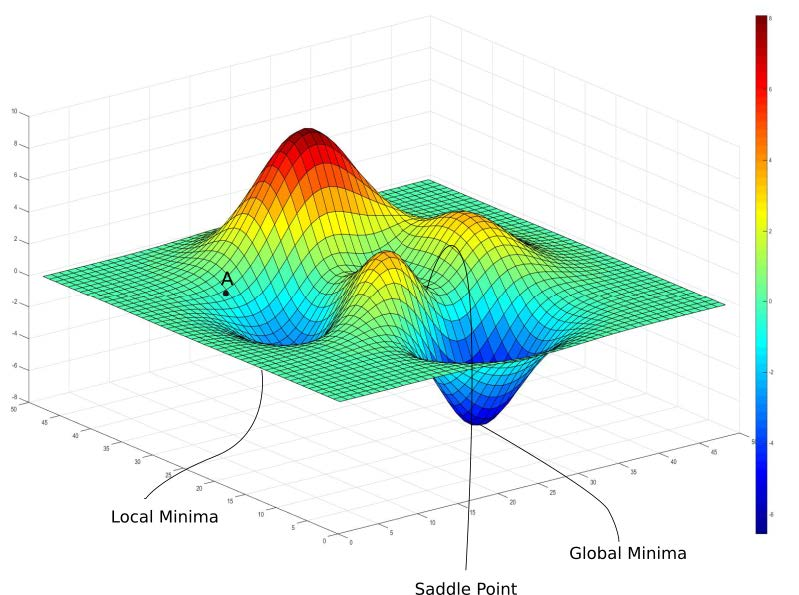
\includegraphics[width=0.9\textwidth]{images/nonconvex_function}
    \caption[A non-convex bivariate function]{A non-convex bivariate function. Taken from \cite{nonconvex_function_img}}
    \label{fig:nonconvex_function}
\end{figure}

A common problem that arises when using gradient descent on a non-linear objective function is that iterates may converge to a local minimum of $J$, especially when the initial point $\mathbf{x}_0$ is already closer to a local minimum than a global one. This issue can be avoided by resorting to other iterative methods which are more robust to the initialization of the starting point, e.g. stochastic gradient descent (sec. \ref{sec:sgd}).

\subsection{Stochastic gradient descent}
\label{sec:sgd}
In machine learning, the cost function $J$ to be minimized is often built upon a dataset $\mathcal{D} = \{(\mathbf{x}_1,y_1),\dots,(\mathbf{x}_N,y_N)\}$ and has the form
\begin{equation}
J(\bm{\theta};\mathcal{D}) = \frac{1}{N} \sum_{i=1}^N \ell(\bm{\theta};\mathbf{x}_i,y_i) + R(\bm{\theta})
\end{equation}
where $R$ is a regularization term and the function $\ell$ in each summand is commonly known as \textit{loss function}, and is parametrized only by a single data point $(\mathbf{x}_i,y_i)$. For instance, the mean squared error (MSE) is a cost function which uses the squared difference between the predicted value $\hat{y}=f(\mathbf{x};\bm{\theta})$ and the real value $y$ as loss function: $\ell(\bm{\theta}; \mathbf{x}, y) = (f(\mathbf{x};\bm{\theta}) - y_i)^2$.

\textbf{Stochastic gradient descent} (SGD) \cite{sgd} is a variant of the gradient descent method in which at each iteration the cost function to be minimized is constructed only on a random subset $\mathcal{B}$ of $\mathcal{D}$ (called \textit{minibatch}). This constitutes a stochastic approximation of the loss function. The size of each minibatch is an hyperparameter; a higher batch size ensures a better approximation of $J$ (which therefore exhibits approximately the same minima of $J$), but determines a slower convergence due to the additional computational cost of computing the gradient. A \textit{training epoch} (or simply \textit{epoch}) refers to one sweep through the entire training set; therefore, a training epoch consists of $\ceil{|\mathcal{D}|/|\mathcal{B}|}$ iterations of the method\footnote{There are $|\mathcal{D}|$ mod $|\mathcal{B}|$ samples left out from any minibatch; a typical choice is to ignore them during the current epoch}. At each epoch, the samples of each minibatch are randomly sampled from $\mathcal{D}$ without replacement. Iterations halt at the end of a user-specified number of epochs, or when other stopping criteria are met (e.g. the learning rate goes below a user-defined threshold).

SGD has several benefits over simple gradient descent:
\begin{itemize}
    \item SGD is more robust to the initialization of $\mathbf{x}_0$ than gradient descent, since the varying cost function at each iteration ensures that the method is less likely to get stuck in local minima.
    \item SGD typically requires more iterations than gradient descent to converge to a minimum, but a single iteration of SGD is computationally cheaper than those of gradient descent. Overall, SGD is faster than gradient descent in terms of computational time, especially when $\mathcal{D}$ is large.
    \item SGD can handle very large training sets, because during each iteration only a minibatch of data must be stored in memory.
\end{itemize}

Gradient descent and SGD are visually compared in fig. \ref{fig:gd_vs_sgd}

\begin{figure}[htb!]
\centering
\begin{subfigure}[t]{0.475\textwidth}
    \centering
    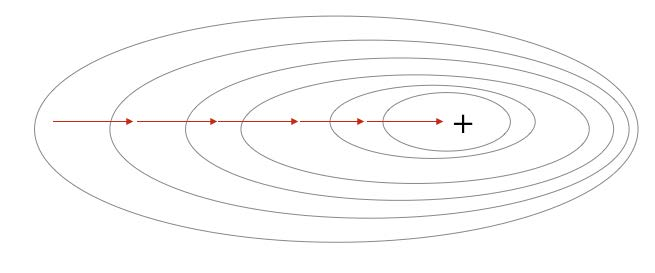
\includegraphics[width=\textwidth]{images/gd}
    \caption{}
\end{subfigure}
\hfill
\begin{subfigure}[t]{0.475\textwidth}
    \centering
    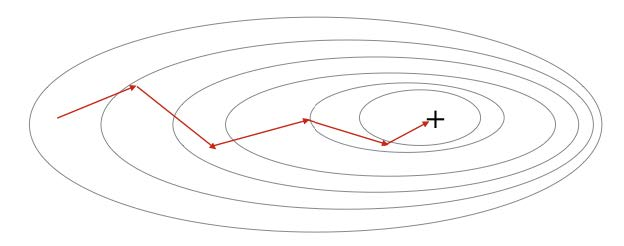
\includegraphics[width=\textwidth]{images/sgd}
    \caption{}
\end{subfigure}
\caption[Minimizing a function through GD and SGD]{Minimizing a bivariate function through (a) gradient descent (b) stochastic gradient descent. Taken from \cite{gd_images}}
\label{fig:gd_vs_sgd}
\end{figure}

\subsubsection{SGD with momentum}
\textbf{SGD with momentum} (SGD-M) \cite{sgd-m} is a variant of the standard SGD method. It changes the usual iterative update of gradient descent and SGD to
\begin{align}
\mathbf{v}_{k+1} &= -\eta \nabla J(\mathbf{x}_k) + \mu \mathbf{v}_k \\
\bm{\theta}_{k+1} &= \bm{\theta}_k + \mathbf{v}_{k+1}
\end{align}
with $\mathbf{v}_0=0$ and where factor $\mu \in (0,1)$ is an hyperparameter. The term $\mathbf{v}_k$ is called \textit{momentum}. This "perturbation" to the direction along which to perform the update has the effect of preserving some information about the previously chosen directions\footnote{The term "momentum" has a meaning similar to that of momentum in physics: when an object is moving it is said to possess momentum, i.e. the product between its mass and (vectorial) velocity; if a force is applied to the object in a generic direction, the object gains momentum in that direction, losing the momentum it already possessed only due to friction. Similarly, in an update of the SGD with momentum we can view $-\nabla J(\bm{\theta}_k)$ as a force which gives the iterates "momentum" along its direction, and this momentum is preserved "by inertia", making the descent path more stable in comparison to that of SGD.} and performing an update also in those directions, ultimately making the descent path less noisy than standard SGD. A visual interpretation of SGD-M is reported in fig. \ref{fig:sgd-m}.

\begin{figure}[hbt!]
    \centering
    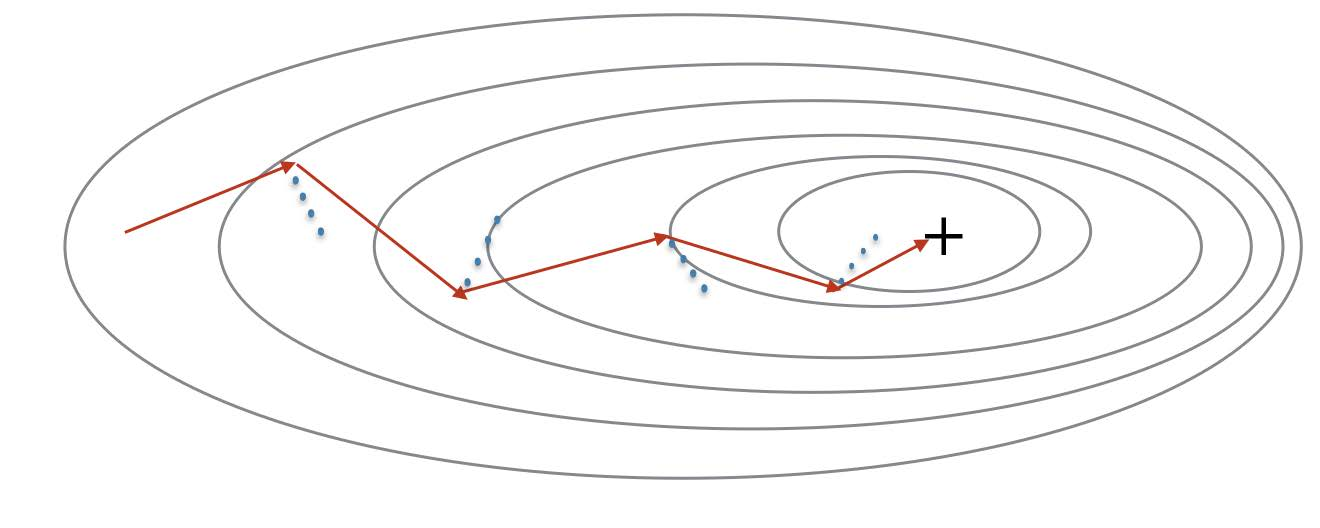
\includegraphics[width=0.475\textwidth]{images/sgd-m}
    \caption[Minimizing a function through SGD-M]{Minimizing a bivariate function through stochastic gradient descent with momentum. Taken from \cite{gd_images}}
    \label{fig:sgd-m}
\end{figure}



\subsection{Nelder-Mead method}
\label{sec:nelder_mead}
\textbf{Nelder-Mead method} \cite{nelder_mead} is a derivative-free iterative method for solving optimization problems. It is useful when we know how to compute the value of the objective function $J$ but not how to evaluate its gradient (or when the gradient is too computationally expensive to compute).

Nelder-Mead method is based on the concept of \textit{simplex}.
\begin{definition}[Simplex]
A $n$-dimensional simplex $\mathcal{S}$ is the convex hull of $n+1$ points $\mathbf{x}_i \in \mathbb{R}^n$, i.e.
\[
\mathcal{S} = \left\{\mathbf{y}\in\mathbb{R}^n \; \middle| \; y=\sum_{i=1}^{n+1} \lambda_i \mathbf{x}_i, \; \lambda_i \geq 0, \; \sum_{i=1}^{n+1}\lambda_i = 1\right\}
\]
The points $\mathbf{x}_i$ ($i=1,\dots,n+1$) are called vertices of $\mathcal{S}$.
\end{definition}
$\mathcal{S}$ is said to be non-singular if $\mathbf{x}_2 - \mathbf{x}_1$, \dots, $\mathbf{x}_{n+1} - \mathbf{x}_1$ are linearly independent. For instance, a line segment is a non-singular simplex in $\mathbb{R}^1$, a triangle in $\mathbb{R}^2$, a tetrahedron in $\mathbb{R}^3$ and so on.

The basic idea of Nelder-Mead method is to start with a given simplex $\mathcal{S}_0$ and modify it at each iteration ($\mathcal{S}_1, \mathcal{S}_2, \dots$) until a suitable simplex is found which provides a good approximation of the optimal solution of the problem.

A generic iteration $k$ of the method is taken from \cite{nelder_mead_implementation} and reported hereafter. Let $\mathcal{S}_k$ be a given non-singular simplex and let $\mathbf{x}_1^{(k)}, \dots, \mathbf{x}_{n+1}^{(k)}$ be its vertices. Assume that the vertices are ordered in such a way that $f(\mathbf{x}_1^{(k)}) \leq \dots \leq f(\mathbf{x}_{n+1}^{(k)})$ (so $\mathbf{x}_1$ is the "best" point of the simplex and $\mathbf{x}_{n+1}^{(k)}$ is the "worst"). We perform the following steps sequentially:

\begin{enumerate}
    \item \textbf{Ordering phase}\\
    Evaluate $f$ at the $n+1$ vertices of $\mathcal{S}_k$ and order the values $f(\mathbf{x}_i^{(k)})$ in increasing order ($f(\mathbf{x}_1^{(k)}) \leq \dots \leq f(\mathbf{x}_{n+1}^{(k)})$), and correspondingly order the vertices of $\mathcal{S}_k$.
    \item \textbf{Reflection phase}\\
    Let $\mathbf{\overline{x}}^{(k)} = \frac{1}{n}\sum_{i=1}^n \mathbf{x}_i^{(k)}$ be the barycenter of the $n$ best points and compute a reflection $\mathbf{x}_R^{(k)}$ of $\mathbf{x}_{n+1}^{(k)}$ w.r.t. $\overline{\mathbf{x}}^{(k)}$:
    \[
    \mathbf{x}_R^{(k)} = \overline{\mathbf{x}}^{(k)} + \rho (\overline{\mathbf{x}}^{(k)} - \mathbf{x}_{n+1}^{(k)})
    \]
    If $f(\mathbf{x}_1^{(k)}) \leq f(\mathbf{x}_R^{(k)}) \leq f(\mathbf{x}_n^{(k)})$, then we accept $\mathbf{x}_R^{(k)}$ as a new vertex of $\mathcal{S}_{k+1}$ in place of $\mathbf{x}_{n+1}^{(k)}$ and go back to step 1, else go to step 3.
    \item \textbf{Expansion phase}\\
    If $f(\mathbf{x}_R^{(k)}) < f(\mathbf{x}_1^{(k)})$ then compute an expansion $\mathbf{x}_E^{(k)}$ as
    \[
    \mathbf{x}_E^{(k)} = \overline{\mathbf{x}}^{(k)} + \chi (\mathbf{x}_R^{(k)} - \overline{\mathbf{x}}^{(k)})
    \]
    else go to step 4.
    If $f(\mathbf{x}_E^{(k)}) < f(\mathbf{x}_R^{(k)})$ then we accept $\mathbf{x}_E^{(k)}$ as a new vertex of $\mathcal{S}_{k+1}$ in place of $\mathbf{x}_{n+1}^{(k)}$ and go back to step 1. Otherwise accept $\mathbf{x}_R^{(k)}$ as a new vertex of $\mathcal{S}_{k+1}$ in place of $\mathbf{x}_{n+1}^{(k)}$ and go back to step 1.
    \item \textbf{Contraction phase}\\
    Compute a contraction $\mathbf{x}_C^{(k)}$ between $\overline{\mathbf{x}}^{(k)}$ and the best among $\mathbf{x}_R^{(k)}$ and $\mathbf{x}_{n+1}^{(k)}$ as
    \[
    \mathbf{x}_C^{(k)} =
    \begin{dcases}
        \overline{\mathbf{x}}^{(k)} - \gamma (\overline{\mathbf{x}}^{(k)} - \mathbf{x}_{n+1}^{(k)}) & \text{if } \mathbf{x}_{n+1}^{(k)} < \mathbf{x}_n^{(k)}\\
        \overline{\mathbf{x}}^{(k)} - \gamma (\overline{\mathbf{x}}^{(k)} - \mathbf{x}_R^{(k)}) & \text{otherwise}\\
    \end{dcases}
    \]
    If $f(\mathbf{x}_C^{(k)}) < f(\mathbf{x}_{n+1}^{(k)})$ then we accept $\mathbf{x}_C^{(k)}$ as a new vertex of $\mathcal{S}_{k+1}$ in place of $\mathbf{x}_{n+1}^{(k)}$ and go back to step 1. Else go to step 6.
    \item \textbf{Shrinking phase}\\
    Compute
    \[
    \mathbf{x}_i^{(k)} = \mathbf{x}_1^{(k)} + \sigma (\mathbf{x}_i^{(k)} - \mathbf{x}_1^{(k)}) \qquad \forall i=2,\dots,n+1
    \]
    and go back to step 1.
\end{enumerate}

A generic iteration of the Nelder-Mead method is visualized in fig. \ref{fig:nelder_mead}.

\begin{figure}[hbt!]
    \centering
    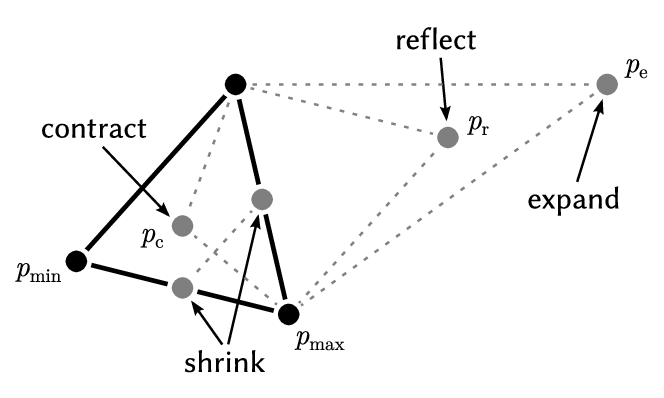
\includegraphics[width=0.6\textwidth]{images/nelder_mead}
    \caption[An iteration of the Nelder-Mead method]{An iteration of the Nelder-Mead method applied to a function $J:\mathbb{R}^2 \to \mathbb{R}$. Taken from \cite{wiki:nelder_mead}}
    \label{fig:nelder_mead}
\end{figure}

The method ends when a stopping criterion is met (e.g. maximum number of iterations reached or when $\norm{f(\mathbf{x}_{n+1}^{(k)}) - f(\mathbf{x}_{1}^{(k)})}$ is below a user-defined threshold). This method is based on the following 4 hyperparameters:
\begin{itemize}
    \item $\rho$: reflection parameter ($\rho>0$)
    \item $\chi$: expansion parameter ($\chi>1, \chi>\rho$)
    \item $\gamma$: contraction parameter ($0<\gamma<1$)
    \item $\sigma$: shrinking parameter ($0<\sigma<1$)
\end{itemize}
Typical choices are: $\rho=1$, $\chi=2$, $\gamma=1/2$, $\sigma=1/2$ \cite{nelder_mead_implementation}. 

The choice of the initial simplex $\mathcal{S}_0$ is also critical. In fact, an initial simplex that is too small can lead to a local search, and in this case the Nelder-Mead method can get more easily stuck.

Although there are no known convergence guarantees for Nelder-Mead method, it is nonetheless widely used because it is computationally cheap and does not require that $J$ is differentiable (continuity is enough).





\section{Time series}
\label{sec:time_series}
Monitoring a driving session of an EV means measuring and recording physical quantities such as vehicle speed, battery voltage, current, SOC and temperature over time. From a mathematical perspective, these discrete-time physical signals, along with the timestamps at which the measurements have been taken, can be treated as a multivariate time series.

\begin{definition}[Time series]
\label{def:ts}
A time series $S$ is an ordered collection of $T$ pairs of timestamps and tuples of $C$ measurements
\[
S=\{(t_1,\mathbf{s}_1),(t_2,\mathbf{s}_2),\dots,(t_T,\mathbf{s}_T)\}
\]
where $t_i \in \mathbb{R}^+$ and $\mathbf{s}_i \in \mathbb{R}^C$.
\end{definition}
It follows that a time series can be thought of as a $C\times T$ matrix.

The number of timestamps, $T$, is also called \textit{length} of the time series, and the number of measurements taken at each timestamp, $C$, is also known as the \textit{number of channels} (or \textit{dimensions}) of the time series; if $C=1$, the time series is \textit{univariate}, whereas if $C>1$ it is \textit{multivariate}. The ordered set of timestamps $t_1,\dots,t_T$ is called \textit{time base} of the time series.\footnote{Def. \ref{def:ts} doesn't take into account those multivariate time series for which each channel has a different time base. However, we can still use the above definition by fixing a "shared" time base (the ordered union of the $C$ different time bases) and opportunely adding \textit{null} values where measurements are not available.} If the time series has an unevenly spaced time base, it is called \textit{unevenly spaced} time series.

An example of a 4-channel multivariate time series (extracted from a real set of EV monitoring data, chap. \ref{sec:aviloo_ds}) is visualized in fig. \ref{fig:ts_example}.

\begin{figure}[hbt!]
    \centering
    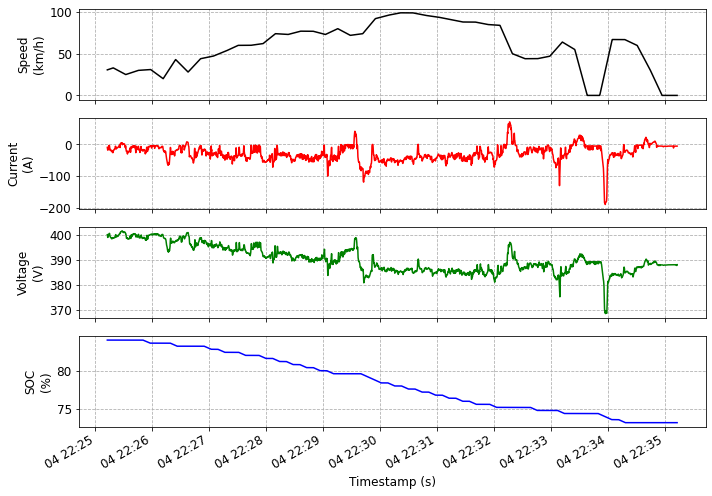
\includegraphics[width=\textwidth]{images/ts_example}
    \caption[A multivariate time series with 4 channels]{A multivariate time series with $C=4$ channels.}
    \label{fig:ts_example}
\end{figure}

Many time windows of monitoring data, along with the SOH value of the battery pack at the particular time the vehicle was driven, form a time series dataset.
\begin{definition}[Time series dataset]
\label{def:ts_ds}
A time series dataset $D$ is a collection of $N$ instances (or \textit{samples})
\[
D = \{(S_1,y_1), (S_2,y_2), \dots, (S_N,y_N)\}
\]
where $S_i$ is a time series and $y_i$ is a scalar value (called \textit{ground-truth label}, \textit{target variable}, \textit{response variable} or \textit{observation}).
\end{definition}
The collection of time series composing the dataset, ($S_1,\dots,S_N)$, can be thought of as a $N \times C \times T$ tensor.

\subsection{Time series extrinsic regression}
\label{sec:tser}
Time series datasets often show up in experimental settings. For this reason, in the past decade there has been an increasing interest in time series analysis research \cite{TSER}. Common tasks in time series analysis are:
\begin{itemize}
    \item Time series classification (TSC): the problem of assigning a label, taken from a finite discrete label set, to a time series
    \item Time series forecasting (TSF): the problem of predicting future values of a time series based on the past measurements; also known as time series regression (TSR)
    \item Time series extrinsic regression (TSER): the problem of assigning a scalar value to a time series
\end{itemize}

TSER is a generalization of both TSC and TSF. The difference between TSER and TSC is that the value to predict is discrete and categorical in TSC, and continuous in TSER; the difference between TSER and TSF is that in TSF the scalar value to predict is some future measurement of the time series, whereas in TSER this assumption is relaxed.

We may frame the problem of predicting the SOH of the battery pack of an EV as a TSER problem: we seek to find a mapping from a time series of driving session monitoring data (with channels such as voltage, current, SOC, temperature, etc.) to the SOH of the battery pack (a scalar in the range [0,100]). In the context of machine learning, such a mapping is also called a \textit{regression model}.

\subsection{Time series feature extraction}
In many experimental settings, the length of the recorded time series is too long in order to train a regression model directly on raw time series data: this is because each measurement is regarded as a feature, and many machine learning algorithms do not scale well with the number of features of a dataset \cite{ts_feat_extr}. Moreover, measurements taken at contiguous timestamps are typically correlated in some way, when dealing with continuous signals, meaning that some sort of feature selection is desirable to reduce this redundancy.

Therefore, it is often preferable to find a static feature-based representation of a time series \cite{ts_feat_extr}. In other words, we may want to find a way to transform a $N\times C\times T$ time series dataset into a static $N\times M$ features dataset (see fig. \ref{fig:ts_feat_extr}), and then train a regression model on this new dataset. These approaches to TSER problems are called \textit{feature-based} regression algorithms \cite{TSER}.

\begin{figure}[hbt!]
    \centering
    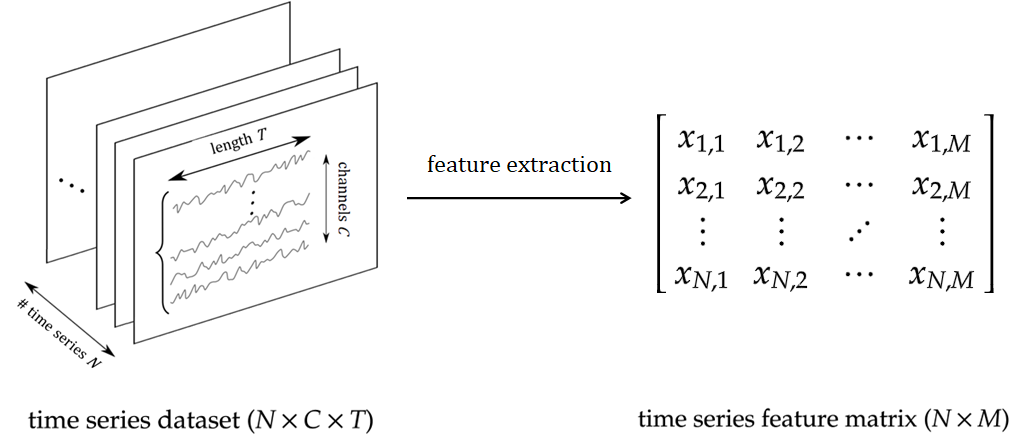
\includegraphics[width=\textwidth]{images/ts_feat_extr}
    \caption{Time series feature extraction}
    \label{fig:ts_feat_extr}
\end{figure}

Time series data differs from static data, which instead is not characterized by a temporal dimension. Since measurements in a time series are correlated in the temporal dimension, generally we cannot use feature extraction techniques commonly used for static datasets, as they are typically not able to capture temporal relationships in data \cite{ts_feat_extr}.

Time series feature extraction methods can be categorized into:
\begin{itemize}
    \item Manual feature extraction: features are hand-crafted by a domain expert to capture relevant information of a specific problem. These domain-specific features are very relevant and discriminative for the problem at hand, but are often poorly generalizable to other regression problems.
    \item Automatic feature extraction: features are automatically extracted by an algorithm, in a supervised or unsupervised fashion (i.e. with or without the knowledge of the label associated to each time series in the dataset). Automatic feature extraction has the advantage of not requiring expertise of the data.
\end{itemize}

The majority of scientific papers on SOH estimation of Li-ion battery cells profusely exploit hand-engineered features \cite{tesi_filippo, manual_extr_soh_2, manual_extr_soh_3, manual_extr_soh_4, manual_extr_soh_5, manual_extr_soh_6, manual_extr_soh_7, manual_extr_soh_8, manual_extr_soh_9, manual_extr_soh_10, manual_extr_soh_11, manual_extr_soh_12, manual_extr_soh_13}, but recent developments point in the direction of automatic feature learning and extraction based on deep convolutional neural networks \cite{auto_extr_soh_1, auto_extr_soh_2, auto_extr_soh_3, auto_extr_soh_4, auto_extr_soh_5}; in the latter approach, the feature extraction step is integrated in the convolutional part of the network (meaning that feature extraction and model training are performed in parallel).

In this thesis work, automatic approaches to feature extraction are explored. Specifically, a recent domain-agnostic unsupervised feature extraction method called \textsc{MiniRocket} is studied (sec. \ref{sec:minirocket}) and applied to our SOH estimation problem. Moreover, a novel computationally-inexpensive feature extraction method has been developed (sec. \ref{sec:my_method}) and applied, achieving surprisingly high performance on a synthetic dataset of monitoring data. The two estimation strategies are thoroughly compared in sec. \ref{sec:results}.





\section{Feature extraction through \textsc{MiniRocket}}
\label{sec:minirocket}
In 2020, Dempster et al. \cite{rocket} proposed \textsc{Rocket}, a new time series classification procedure that achieves state-of-the-art accuracy in TSC with a low computational expense. \textsc{Rocket} consists of two parts: an unsupervised feature extraction step which transforms time series using a large number of random convolutional kernels, and a classification step with a classification model of choice (by default a ridge regression classifier).
One year later, the same authors reformulated \textsc{Rocket} into a new classification method, called \textsc{MiniRocket} (for \textbf{MINI}mally \textbf{R}and\textbf{O}m \textbf{C}onvolutional \textbf{KE}rnel \textbf{T}ransform) \cite{minirocket}. It is up to 75 times faster than \textsc{Rocket}, while being almost fully deterministic and maintaining essentially the same performances on TSC tasks.

By replacing \textsc{MiniRocket}'s classification model with a regression model, \textsc{MiniRocket} becomes a time series regression algorithm, which is able to achieve state-of-the-art performances in TSER problems \cite{TSER}.

We will now briefly describe how \textsc{MiniRocket}'s feature extraction step works when dealing with univariate time series datasets. A naive extension to multivariate time series is then described.



\subsection{Convolution}
\label{sec:convolution}
Convolution is a widely used transformation applied to a matrix, which consists in computing a locally weighted sum of its elements with weights given by a matrix called \textit{kernel}.

\begin{definition}[Discrete 2D convolution]
Given a matrix $X \in \mathbb{R}^{n\times m}$ (called \textit{input feature map}) and a matrix $W \in \mathbb{R}^{h\times k}$ (called \textit{convolutional kernel}), the discrete 2D convolution (or simply convolution) between $X$ and $W$ is the matrix $Z$ (called \textit{output feature map}) whose elements are given by the following operation
\[
Z(i,j) = (X*W)(i,j) = \sum_{r=1}^h \sum_{s=1}^k X(i+s-1, j+r-1) W(r, s)
\]
\end{definition}
Usually, a bias value $b\in\mathbb{R}$ is added to the convolution output in many applications.

\begin{remark}
When $m=k=1$, the discrete convolution becomes 1-dimensional. This is the operation applied to univariate time series (which can be thought of as $1\times T$ matrices, or equivalently as vectors of length $T$).
\end{remark}

Convolution has a simple visual interpretation, visualized in fig. \ref{fig:convolution}: the kernel matrix "slides" over the input feature map vertically and horizontally, locally identifying a submatrix on the input feature map of the same shape as the kernel; the elements of the output feature map are computed by taking the element-wise product of the kernel and said submatrix and summing them.

\begin{figure}
    \centering
    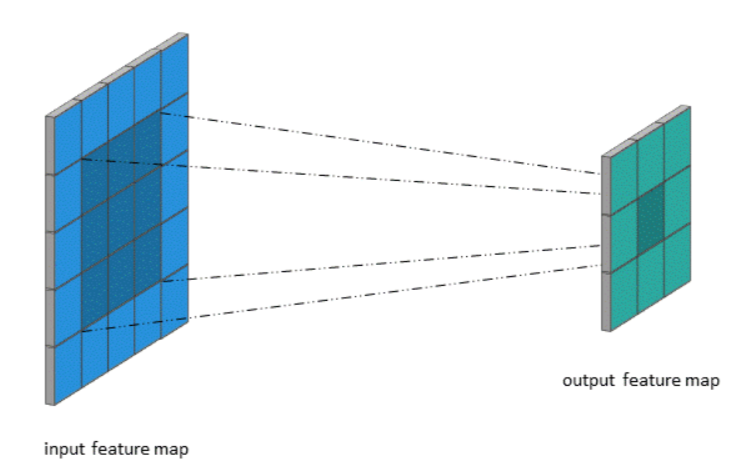
\includegraphics[width=0.6\textwidth]{images/convolution}
    \caption[Discrete convolution]{A visual representation of a discrete 2D convolution between a $5\times5$ input feature map and a $3\times3$ kernel. Taken from \cite{conv_fig}}
    \label{fig:convolution}
\end{figure}

In many applications, richer variants of the convolution operation are used, which employ the techniques of \textit{zero-padding} and \textit{dilation} \cite{dl_book}:

\begin{itemize}
\item Zero-padding (or simply padding) consists in concatenating rows/columns full of zeros at the beginning or the end of an input feature map, prior to applying convolution. typically, the number of leading and trailing rows/columns added is the same ($p$). A zero-padded convolution is visualized in fig. \ref{fig:padded_conv}
\item Dilation consists in "spreading" a kernel over the input feature map, such that with a dilation parameter of $d$ the weights in a kernel are convolved with every $d$-th element of an input feature map along each direction. A dilated convolution is visualized in fig. \ref{fig:dilated_conv}.
\end{itemize}

\begin{figure}[htb!]
\centering
\begin{subfigure}[t]{0.45\textwidth}
    \centering
    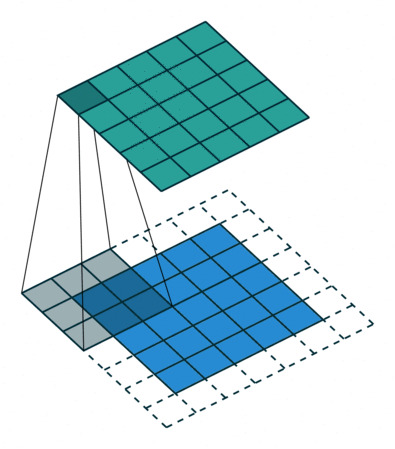
\includegraphics[width=\textwidth]{images/padded_conv}
    \caption[Zero-padded convolution]{Zero-padded convolution with padding parameter $p=1$}
    \label{fig:padded_conv}
\end{subfigure}
\hfill
\begin{subfigure}[t]{0.45\textwidth}
    \centering
    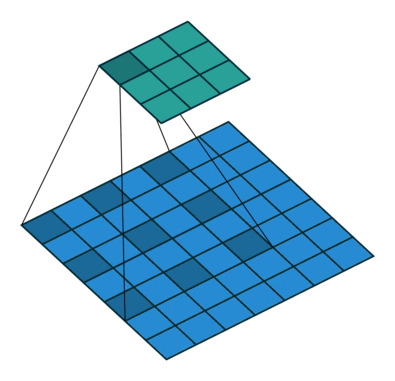
\includegraphics[width=\textwidth]{images/dilated_conv}
    \caption[Dilated convolution]{Dilated convolution with dilation parameter $d=2$}
    \label{fig:dilated_conv}
\end{subfigure}
\caption[Variants of the convolution operation]{Variants of the convolution operation between a $5\times5$ input feature map and a $3\times3$ kernel. Taken from \cite{conv_variants_fig}}
\label{fig:conv_variants}
\end{figure}



\subsection{Fitting \textsc{MiniRocket}'s feature extractor}
\label{sec:minirocket_feat_extr}


\paragraph{Length}
\textsc{MiniRocket} uses a fixed set of 84 kernels of length 9, with weights restricted to two values. These 84 kernels are selected a priori among the $2^9=512$ possible two-valued kernels of length 9. Using such a low number of kernels helps in keeping the computational cost low enough while not hampering performances.


\paragraph{Weights}
The 84 chosen kernels have weights restricted to two values: $\alpha=-1$ and $\beta=2$. This choice is made arbitrarily by the authors, in the sense that the scale of these values is unimportant, as bias values are drawn from the convolution output (as discussed in the next paragraph) and so they match its very scale. Thus, it is not necessary to normalise the input time series.

Moreover, the number of -1s is double the number of 2s in all 84 kernels, such that the sum of the weights of a kernel is 0. This ensures that the kernels are sensitive only to the \textit{relative} magnitude of the input values, i.e. that the convolution output is invariant to the addition or subtraction of any constant value to the input: $X*W = (X\pm c)*W$.

The position of the three $\beta=2$ weights inside each of the 84 kernels is defined by the sequence $[(1,2,3), (1,2,4), \dots, (6,8,9), (7,8,9)]$.


\paragraph{Bias}
Bias values associated to each kernel/dilation combination are used in computing PPV features, as discussed in the associated paragraph.
For a given kernel $W$ and dilation parameter $d$ (in short: $W_d$), bias values are drawn from the quantiles of the convolution output between $W_d$ and a randomly selected time series $X_i$ in the dataset. The orders of the quantiles assigned to each $W_d$ are computed deterministically with the following low-discrepancy sequence
\begin{equation}
i\cdot\frac{1+\sqrt{5}}{2}\text{ mod }1,\;\forall i\in [1,2,\dots,n]
\end{equation}
where $n$ is the total number of desired PPV features to be extracted.

The number of biases to use with each kernel/dilation combination $W_d$ (or, equivalently, the number of features that are extracted from the convolution output with kernel/dilation $W_d$) depend on $d$ and on the length $l$ of the time series $X$, as discussed in the next paragraph.

Drawing at random a time series $X_i$ for the purpose of sampling the bias values is the only stochastic element of \textsc{MiniRocket}; remaining parameters either depend solely on the time series length or are intended to be kept at their default values.


\paragraph{Dilation}
Possible dilation for each kernel values are in the range
\begin{equation}
D=\{\floor{2^0},\floor{2^{\text{max}/m}},\floor{2^{2\cdot\text{max}/m}},\dots,\floor{2^{m\cdot\text{max}/m}}\}
\end{equation}
where $m$ is the maximum possible number of dilations per kernel (set to 32 by default) and $\text{max}=\log_2(l-1)/8$ is the largest possible dilation parameter for a kernel of length $9$ applied to a time series of length $l$ (i.e. such that the \textit{effective} length of the dilated kernel of length $9$ is exactly $l$).

The count of each unique integer dilation value in $D$ determines the number of PPV features to be computed per dilation (scaled according to the total number of desired PPV features, $n$, so that the sum of the scaled counts equals $n$), ensuring that exponentially more features are computed for smaller dilations.


\paragraph{Padding}
Zero-padding is applied alternately every other kernel/dilation combination such that, overall, half the combinations use padding and half do not. The number of leading and trailing zeros added to the time series is set in such a way that the convolution operation begins with the middle (5th) weight of a kernel centered on the first measurement of the time series and ends with the middle weight centered on the last measurement.


\paragraph{Features}
The feature extracted by \textsc{MiniRocket} from each time series $X$ for each kernel/dilation combination $W_d$ and each bias $b$ is the proportion of convolution output values which are greater than $b$:
\begin{equation}
\text{PPV}(X*W_d, b) \coloneqq \frac{1}{n_\text{out}} \sum\left[X*W_d > b\right]
\end{equation}
where $n_\text{out}$ denotes the number of elements of the convolution output vector $X*W_d$ and $[\mathbf{x}\in a]$ denotes the indicator function. PPV stands for \textit{proportion of positive values}.

By default, \textsc{MiniRocket} represents each time series with a total of 9,996 PPV features (i.e. the nearest multiple of 84 -- the number of kernels -- less than 10,000).


\subsection{\textsc{MiniRocket} for multivariate time series}
\label{sec:multivariate-minirocket}
The authors \cite{minirocket} also extended \textsc{MiniRocket} to multivariate time series in a basic way\footnote{The explanation of multivariate \textsc{MiniRocket} given in this section is based only on the code implemented by the authors (which can be found at \url{https://github.com/angus924/minirocket/blob/main/code/minirocket_multivariate.py}), as the extension to multivariate time series is not mentioned anywhere in the original paper \cite{minirocket}.}.

Suppose that the time series in the dataset have $C$ channels. For each kernel/dilation combination, a random subset of $k = \floor{2^{\mathcal{U}(0,M)}}$ out of $C$ channels is taken, where $M = \log_2(\min(C,9)+1))$ and $\mathcal{U}(0,M)$ means taking a random sample from the uniform distribution on $(0,M)$.\footnote{$k$ is distributed according to the floor of a log-uniform distribution on $[1,M]$.

A random variable $X$ is distributed according to a log-uniform distribution with support on $[a,b]$ if $\ln{(X)}\sim\mathcal{U}(ln(a),ln(b))$, where $\mathcal{U}$ indicates the uniform distribution. \cite{loguniform}

Suppose now that $a,b\in\mathbb{N}$; it can be proved that $\floor{X}$ is a discrete random variable with support on $\{a, a+1, \dots, b-1\}$ with probability mass function
\[
p(n) = \ln\left(\frac{n+1}{n}\right) / \ln\left(\frac{b}{a}\right)
\]
E.g.: when sampling a random subset of $k$ out of $C=3$ channels from a multivariate time series, with $k$ distributed according to the above distribution, the probability masses of $k$ are: $p(1)=0.5$, $p(2)=0.292$, $p(3)=0.208$. Therefore, smaller subsets are more likely to be extracted.
}

When drawing the biases for each kernel/dilation combination, kernel $W_d$ is convolved with each of the $k$ channels of $X$ that have been randomly selected; then, the $k$ convolution outputs are summed, and this vector is used to draw the biases with the procedure already discussed in sec. \ref{sec:minirocket_feat_extr}.

This variant of \textsc{MiniRocket}'s feature extractor for multivariate time series "suffers" from at least two drawbacks with respect to the original, univariate version:
\begin{itemize}
\item A new stochastic element is added: the random sampling of the channels of the time series to be used in the feature extraction, for each kernel/dilation combination.
\item The different channels of a time series do not have the same mean and standard deviation in general. Since the sum of several convolution outputs is taken, the time series channels must be normalized for this method to make sense mathematically (whereas original \textsc{MiniRocket} doesn't require time series to be normalized, as discussed in sec. \ref{sec:minirocket_feat_extr}).
\end{itemize}



\section{Feature selection with PCA}
\label{sec:pca}
Dealing with high-dimensional datasets (i.e. datasets with a large number of predictors) is often undesirable. Many machine learning models do not scale well to high-dimensional datasets due to sparseness in data (a phenomenon known as \textit{curse of dimensionality}) and generally high computational cost. Moreover, predictors have some degree of mutual dependence in many experimental settings. For these reasons, it is often desirable to perform a \textbf{dimensionality reduction} of the data \cite{dim_red}.

\textbf{Principal Components Analysis} (PCA) \cite{pca} is a method for performing a particular change of basis on the data, in which the axes of the new coordinate system are the set of orthonormal eigenvectors of the scatter matrix $A=X^TX$, commonly known as "principal components" of the dataset $X$. PCA is typically exploited as an unsupervised dimensionality reduction technique, since it has the nice property of maximizing the variance of the data when mapped down to lower dimensional spaces.

The PCA problem can be expressed in many different ways, which can be proven to be equivalent. One of the most interesting statements is the following one.

Given a dataset $X\in\mathbb{R}^{N\times M}$, with data points $\mathbf{x}_1, \dots, \mathbf{x}_N$, and assuming that data is zero-centered ($\frac{1}{N}\sum_{i=1}^N \mathbf{x}_i = 0$), find a set of $D \leq M$ orthonormal directions $\mathbf{w}_1,\dots,\mathbf{w}_D$ by solving consecutively the following variance maximization problems:
\begin{align}
\begin{split}
\argmax_{\mathbf{w}_1:\norm{\mathbf{w}_1}=1} \quad & \frac{1}{N}\sum_{i=1}^N(\langle\mathbf{w}_1,\mathbf{x}_i\rangle)^2\\
\argmax_{\substack{\mathbf{w}_k:\norm{\mathbf{w}_k}=1 \\ \mathbf{w}_kA\mathbf{w}_j=0, \; j=1,\dots,k-1}} \; & \frac{1}{N}\sum_{i=1}^N(\langle\mathbf{w}_k,\mathbf{x}_i\rangle)^2, \qquad k=2,\dots,D
\end{split}
\end{align}

This problem is solved by choosing $\mathbf{w}_1=\mathbf{u}_1,\dots,\mathbf{w}_D=\mathbf{u}_D$, where $\mathbf{u}_1,\dots,\mathbf{u}_D$ are the unit-norm eigenvectors associated to the largest $D$ eigenvalues of the scatter matrix $A$; the maximum values of the objective functions of each problem are, in order, $\lambda_1,\dots,\lambda_D$.

This formulation is of particular interest because of the following interpretation: $\mathbf{w}_1$ is the direction of a line onto which the variance of the projected points, $\langle\mathbf{w}_1,\mathbf{x}_i\rangle$, is maximized; $\mathbf{w}_2$, is a second direction which maximizes the variance of $\langle\mathbf{w}_2,\mathbf{x}_i\rangle$ but which is also orthogonal to $\mathbf{w}_1$ (i.e., the projected points onto $\mathbf{w}_1$ and $\mathbf{w}_2$ are uncorrelated); and so on with the remaining maximization problems, which yield other directions of variance maximization which are orthogonal to all the previously found directions. This interpretation is particularly evident in fig. \ref{fig:pca}

\begin{figure}[htb!]
    \centering
    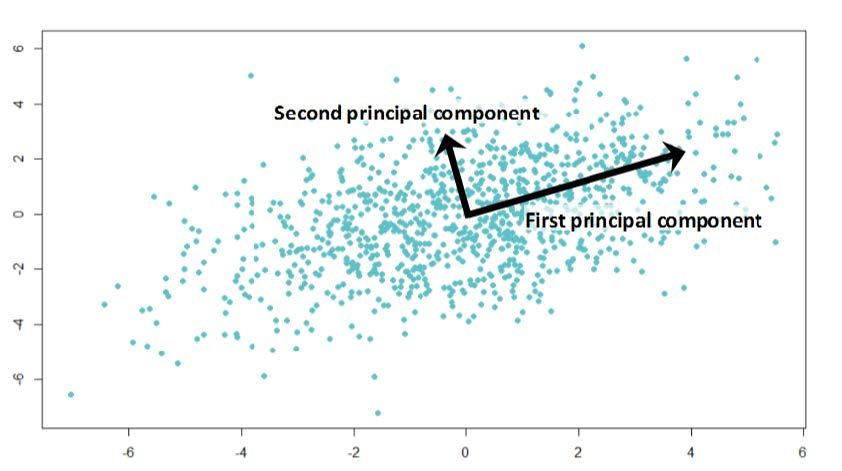
\includegraphics[width=\textwidth]{images/pca}
    \caption[PCA on a 2D dataset]{PCA on a simple 2D dataset. Taken from \cite{pca_img}}
    \label{fig:pca}
\end{figure}

The proportion of the variance represented (or "\textit{explained}") by each eigenvector can be calculated by dividing the eigenvalue corresponding to that eigenvector by the sum of all eigenvalues. This means that by reducing dimensionality with $D$ principal components, the proportion of variance explained by these is $\sum_{i=1}^D \lambda_i / \sum_{i=1}^M \lambda_i$.

Performing dimensionality reduction through PCA is especially useful when using \textsc{MiniRocket} as a feature extractor, since it produces a very large number of features (9,996) from each input time series.





\section{Feature extraction through linear regression in the V-I-SOC space}
\label{sec:my_method}
\textsc{MiniRocket} is a domain-agnostic feature extractor, meaning that it could be effective in many different experimental contexts. However, embedding a SOH estimation method on an EV requires that the procedure has a low memory footprint and -- most critically --
a limited computational cost, due to the need of estimating the SOH in real-time. When performing a SOH prediction, \textsc{MiniRocket} computes almost 10,000 convolutions between the time window of monitoring data given as input and the \textsc{MiniRocket} kernels. As the length of the time windows increase, computing so many convolutions becomes infeasible for the computational devices embedded on a typical BMS of an EV.

In this section, a new feature extraction method is introduced. This method is:
\begin{itemize}
    \item domain-specific: this method is specifically designed for the task of estimating an EV battery pack's SOH; it leverages only on the voltage (V), current (I) and SOC measurements recorded during a driving session and takes the shape of their data distribution into account;
    \item computationally cheap: for each time window of monitoring data, a simple multivariate linear regression model is fitted, an operation which requires only a limited amount of computation;
    \item low dimensional: from each time window of monitoring data only 3 features are extracted.
\end{itemize}

Some preliminary definitions are introduced in order to more easily explain how this method works.

EV field data typically consists of time series of V, I, SOC measurements (among others), taken during a driving session of the vehicle. From now on, we will refer to the tuple of measurements $(\text{V}(t_i), \text{I}(t_i), \text{SOC}(t_i))$ at a timestamp $t_i$ as an \textbf{operating point} of the EV.

The first key observation in the design of this novel procedure is that the operating points observed on a certain driving session seem to lie on a hyperplane in the V-I-SOC space. This observation is very accurate in relation to synthetic data (fig. \ref{fig:visoc_synth1} and \ref{fig:visoc_synth2}), but it is also true for real monitoring data with a certain degree of approximation (fig. \ref{fig:visoc_real1} and \ref{fig:visoc_real2}).

\begin{figure}[htb!]
\centering
\begin{subfigure}[t]{0.475\textwidth}
    \centering
    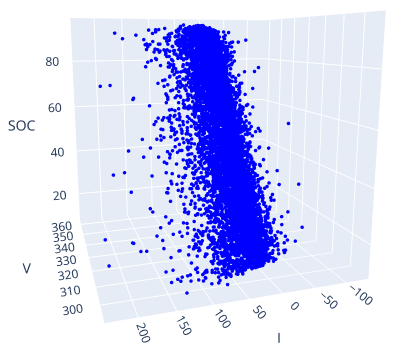
\includegraphics[width=\textwidth]{images/visoc_synth1}
    \caption{}
    \label{fig:visoc_synth1}
\end{subfigure}
\hfill
\begin{subfigure}[t]{0.475\textwidth}
    \centering
    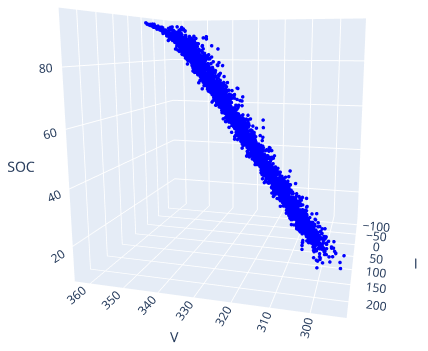
\includegraphics[width=\textwidth]{images/visoc_synth2}
    \caption{}
    \label{fig:visoc_synth2}
\end{subfigure}
\vskip\baselineskip
\begin{subfigure}[t]{0.475\textwidth}
    \centering
    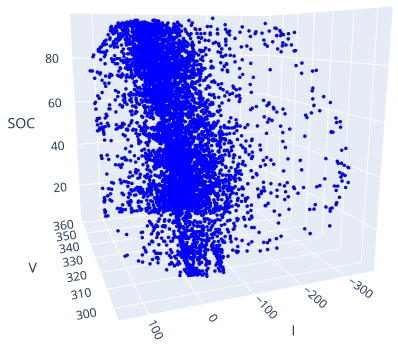
\includegraphics[width=\textwidth]{images/visoc_real1}
    \caption{}
    \label{fig:visoc_real1}
\end{subfigure}
\hfill
\begin{subfigure}[t]{0.475\textwidth}
    \centering
    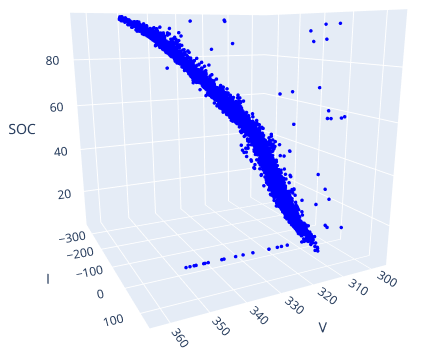
\includegraphics[width=\textwidth]{images/visoc_real2}
    \caption{}
    \label{fig:visoc_real2}
\end{subfigure}
\caption[Synthetic and real operating points associated to the same SOH level]{Operating points associated to the same SOH level, randomly extracted from: (a)-(b) synthetic dataset (sec. \ref{sec:ds_gen}), (c)-(d) real dataset (chap. \ref{sec:aviloo_ds}).}
\label{fig:visoc}
\end{figure}

The particular hyperplane defined by the operating points seems to independent of the particular drive cycle, but interestingly it seems to be discriminative of the age of the battery during that driving session. In fact, the second key observation is that different battery SOH values define different hyperplanes in the V-I-SOC space. This is highlighted in fig. \ref{fig:visoc_soh_planes}.

\begin{figure}
    \centering
    \hspace{-1cm}
    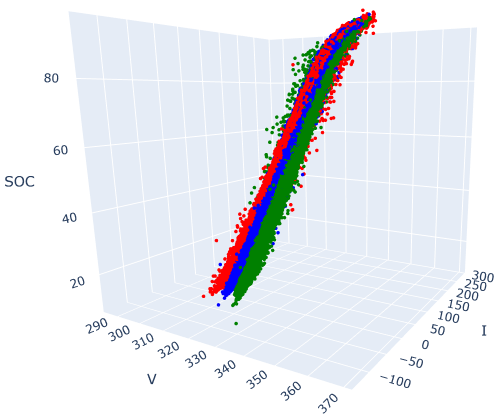
\includegraphics[width=0.7\textwidth]{images/visoc_soh_planes}
    \caption[Synthetic Operating points associated to different SOH levels]{Operating points associated to different SOH levels (red: 100\%, green: 90\%, blue: 80\%), randomly extracted from the synthetic dataset.}
    \label{fig:visoc_soh_planes}
\end{figure}

Therefore, we may argue that the problem of predicting the SOH of a battery pack is equivalent to the task of finding the hyperplane which approximates all the possible operating points of an EV at a specific point of its operating lifetime.

To make this task compatible with the requirements of a real-time SOH estimation method, we need to find said hyperplane from the knowledge of only a relatively short time window of operating points (i.e. a small sample of consecutive operating points) instead of the whole statistical population of operating points.

The equation of an affine hyperplane in a three-dimensional space is
\begin{equation}
    z=ax+by+c
\end{equation}
A 3D hyperplane is uniquely identified by its three parameters $a, b, c \in \mathbb{R}$.

Therefore, we can represent a time window of operating points with just three features, namely the $a, b, c$ parameters defining the hyperplane which better "describes" those operating points.

Estimating the parameters of the hyperplane which passes near all the points in a given set can be stated as a linear regression problem \cite{hastie}.
\begin{definition}[Multiple linear regression model]
\label{def:linear_model}
Let $\mathbf{x}=(x_1,\dots,x_M) \in \mathbb{R^M}$. A multiple linear regression model (or simply linear model) is a function of the form
\[
f(\mathbf{x};\bm{\beta}) = \beta_0 + \sum_{i=1}^M \beta_i x_i
\]
\end{definition}
In many experimental contexts, a linear model is a reasonable approximation of the relationship between an output variable $y$ and an input vector $\mathbf{x}$.

The problem of estimating the parameters $\bm{\beta}$ of a linear model from a set of training data $(\mathbf{x}_{1},y_1),\dots,(\mathbf{x}_{n},y_n)$ is called \textit{linear regression problem}. There exists many estimation methods for solving the linear regression problem. Two such methods have been explored for designing our novel feature extractor: ordinary least squares estimation (sec. \ref{sec:ols}) and Theil-Sen estimation (sec. \ref{sec:theil-sen}).

\subsection{Ordinary least squares estimation}
\label{sec:ols}
Ordinary least squares (OLS) estimation is the most common solver for a linear regression problem. It consists in finding the parameters $\bm{\beta}$ minimizing the residual sum of squares
\begin{equation}
\text{RSS}(\beta) = \sum_{i=1}^N (y_i - f(\mathbf{x}_{i};\bm{\beta}))^2
\end{equation}

Let $X$ the $N\times M+1$ matrix having the dataset samples $\mathbf{x}_{1},\dots,\mathbf{x}_{N}$ as rows, with a constant $x_{i,0}=1$ prepended to each row to account for the bias term, and let $\mathbf{y} = (y_1,\dots,y_N)^T$. The analytical expression of the RSS can be rewritten as
\begin{equation}
\text{RSS}(\bm{\beta}) = \norm{\mathbf{y}-X\bm{\beta}}^2 = (\mathbf{y}-X\bm{\beta})^T(\mathbf{y}-X\bm{\beta})
\end{equation}

If the Gram matrix $X^T X$ is positive definite, then the OLS regression problem has a unique solution:
\begin{equation}
\hat{\bm{\beta}}^{OLS} = (X^TX)^{-1}X^T\mathbf{y}
\end{equation}

The OLS method is visualized in fig. \ref{fig:ols}.

\begin{figure}[hbt!]
    \centering
    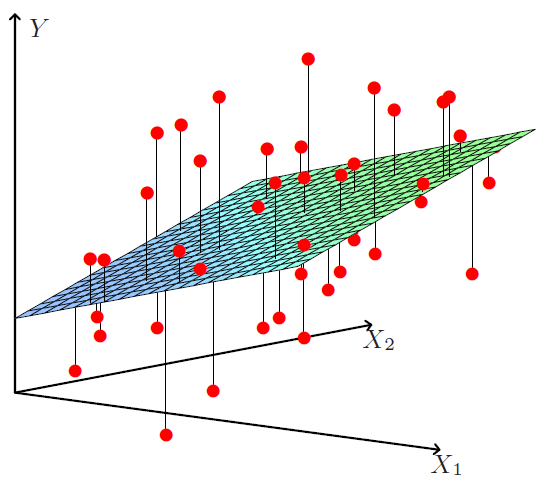
\includegraphics[width=0.7\textwidth]{images/ols}
    \caption[Fitting a linear model via OLS]{Fitting of a linear model on a 2D dataset by ordinary least squares estimation. We seek the linear function of $\mathbf{x}$ that minimizes the sum of squared residuals from $y$. Taken from \cite{hastie}}
    \label{fig:ols}
\end{figure}

OLS generally yields a good estimate for the parameters $\bm{\beta}$ under the assumption that $\mathbb{E}(y|\mathbf{x})$ is a linear function with good approximation. However, OLS estimates are highly sensitive to outliers, since it seeks to minimize all residuals equally and penalizes large residuals more (due to squaring) \cite{robust_regr}. In many experimental contexts the available data is contaminated by outliers, which for instance arise from measurement errors due to sensors (as is often the case in EV monitoring data), approximation errors (as is the case when resampling EV monitoring data to a common time base for all the signals through linear interpolation) or even unavoidable sampling error (which in the EV context is due to the fact that sensors monitor continuous signals by collecting them at a specific sampling rate, therefore often neglecting their sudden high-frequency variations).

Robust regression methods \cite{robust_regr} are designed to limit the effect that the presence of outliers has on regression estimates.

\subsection{Theil-Sen estimation}
\label{sec:theil-sen}
Theil-Sen (TS) estimation method is a robust alternative to the OLS method that reduces outliers' contribution to the error loss, thereby limiting their impact on regression estimates.

TS estimation was first introduced by Henri Theil \cite{theil} and Pranab K. Sen \cite{sen} as a method for fitting simple linear models (i.e. models with just one explanatory variable, $f(x;m,b)=mx+b$); recently, it has been generalized to multiple linear regression by Dang et al. \cite{multi_theil-sen}.

\subsubsection{Theil-Sen estimation for simple linear models}
As originally defined by Theil \cite{theil}, the TS estimate for the slope parameter $m$ of the simple linear model on a set of two-dimensional points $(x_1,y_1),\dots,(x_N,y_N)$ is the median of the slopes $m_{i,j} = (y_j - y_i)/(x_j - x_i)$ determined by all pairs of sample points. Sen \cite{sen} extended this definition to handle the case in which two data points have the same $x$ coordinate, by taking the median of the slopes determined only by pairs of points having distinct $x$ coordinates. The intercept $b$ can be estimated in a number of ways; one of them is setting $b$ as the median of the values $b_i = y_i - \hat{m}^{TS}x_i$.

It is clear that computing $\hat{m}^{TS}$ and $\hat{b}^{TS}$ with this procedure becomes very expensive as the dataset size $N$ increases: for $N$ points, $\binom{N}{2} = \frac{N(N-1)}{2}$ slopes must be computed -- one for each pair of points.

One possible solution is sampling at random a subpopulation $S \ll \binom{N}{2}$ of pairs of points and performing Theil-Sen estimation on this reduced training set, effectively computing only $S$ slopes. This has the effect of reducing the computational cost, but the estimation may become very sensitive to the particular random choice of the subpopulation, especially if $S$ is very small. This variant of the Theil-Sen method is implemented in the Python library scikit-learn, where $S$ is set with the hyperparameter \texttt{max\_subpopulation} \cite{sklearn_theil-sen}. In this thesis work, $S$ has been set to 10,000 for all experiments.

The Theil–Sen estimator is an unbiased estimator for the true slope $m$ \cite{sen, unbiasedness_theil-sen}, has high asymptotic efficiency \cite{sen, efficiency_theil-sen} and is more robust to outliers than OLS estimator \cite{multi_theil-sen}. In its original formulation (simple linear regression and $S=\binom{N}{2}$), it has a breakdown point of 29.3\%, meaning that it can tolerate arbitrary corruption of up to 29.3\% of the input data points without degradation of its accuracy.

A visual comparison between OLS and Theil-Sen estimation applied to a simple 2D dataset with outliers is reported in fig. \ref{fig:theil-sen_vs_ols}.
\begin{figure}[hbt!]
    \centering
    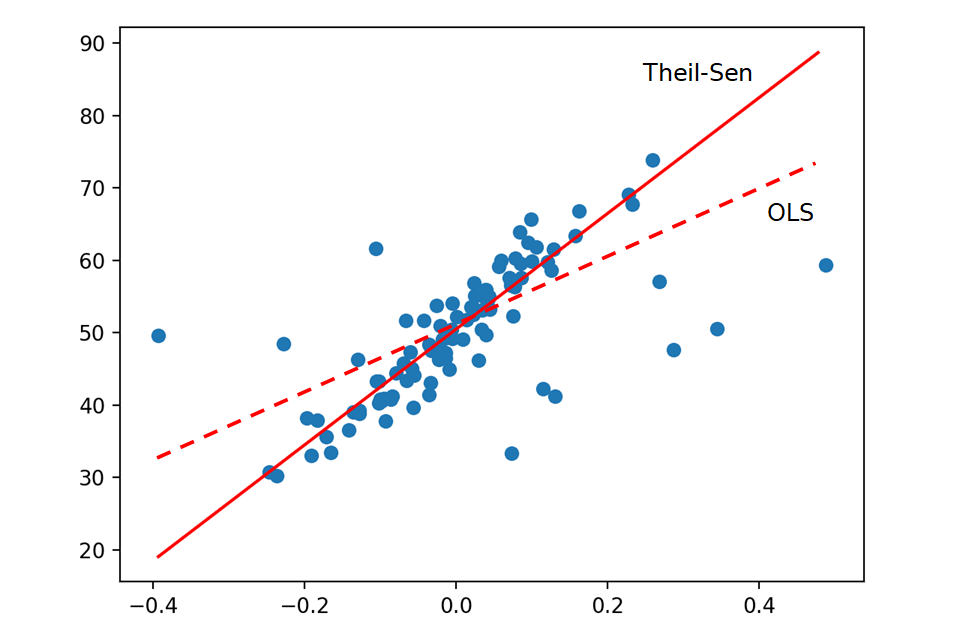
\includegraphics[width=0.8\textwidth]{images/theil-sen_vs_ols}
    \caption[Fitting a simple linear model via TS]{Fitting a simple linear regression model via Theil-Sen estimation vs ordinary least squares. Adapted from \cite{theil-sen_vs_ols}}
    \label{fig:theil-sen_vs_ols}
\end{figure}

On a final note, there is no closed form solution for TS estimates, as opposed to OLS; the algorithmic nature of TS method makes it well-suited for a computer implementation.

\subsubsection{Theil-Sen estimation for multiple linear models}
Recently, Dang et al. \cite{multi_theil-sen} extended Theil-Sen estimation to multiple linear regression.

Consider a multiple linear regression model $f(\mathbf{x};\bm{\beta}) = \bm{\beta}\mathbf{x}$ (where, as usual, $\bm{\beta},\mathbf{x} \in \mathbb{R}^{M+1}$ and $x_{i,0}=1$). The hyperplane defined by the regression parameters $\bm{\beta}$ is determined by exactly $M+1$ points. Similarly to the simple regression case, we can consider a (random) subpopulation of $S\leq \binom{N}{M+1}$ subsets of $M+1$ points ($\mathbf{k}_1, \dots, \mathbf{k}_S$) and compute the unique $\bm{\beta}^{(i)}$ associated to each $\mathbf{k}_i$ by solving the associated OLS problem\footnote{Note that the OLS problem with exactly $n$ points in a $n$-dimensional space is trivially equivalent to finding the (unique) hyperplane passing through those $n$ points.}:
\begin{equation}
\bm{\beta}^{(i)} = (X^{(i)T} X^{(i)})^{-1} X^{(i)T} \mathbf{y}
\end{equation}
where $X^{(i)}$ is the matrix whose rows are the vectors $\mathbf{x}_{j} \in \mathbf{k}_i$. Notice that with this procedure the "slope vector" $(\beta_1^{(i)},\dots,\beta_{M+1}^{(i)})$ and the intercept $\beta_0^{(i)}$ are computed simultaneously.

After having computed $\bm{\beta}^{(1)},\dots,\bm{\beta}^{(S)}$, the Theil-Sen estimate for $\bm{\beta}$ is their sample spatial median \cite{spatial_median}
\begin{equation}
\hat{\bm{\beta}}^{TS} = \text{\textsc{SpatialMedian}}(\bm{\beta}^{(1)},\dots,\bm{\beta}^{(S)})
\end{equation}
For reference, the sample spatial median is discussed in appendix \ref{sec:spatial_median}

Multiple Theil-Sen estimation (MTS) is still robust to outliers, although a bit less than its simple counterpart, with a breakdown point of $1-(1/2)^{1/(M+1)}$. E.g.: for $M+1=3$, as in our experimental setting (see chap. \ref{sec:experiments}), the breakdown point is 20.6\%.





\section{Regression models}
\label{sec:regr_models}
Upon transforming a time series dataset to its static feature-based representation, we must choose and train a regression model to predict the SOH. A huge amount of regression models exist, both linear and non-linear; in this thesis work, we experiment with three well-known regression models: ridge regression (sec. \ref{sec:ridge}), random forest (sec. \ref{sec:random_forest}), feed-forward neural network (sec. \ref{sec:neural_network}).



\subsection{Ridge regression}
\label{sec:ridge}
Consider once more the linear regression model (def. \ref{def:linear_model}). In some cases, the Gram matrix $X^T X$ is singular or nearly-singular: this happens in particular when there are multicollinear (i.e. highly correlated) independent variables in the data. Because the OLS estimates depend upon $(X^T X)^{-1}$, when $X^T X$ is nearly-singular the OLS estimation problem becomes ill-posed, and this may lead to serious numerical problems, namely estimates exhibiting high variance\footnote{For instance, let us suppose that a dataset has two independent variables "weight" and "height" and one dependent variable "age". It is reasonable to assume that weight and height have a strong linear correlation. When fitting a linear model to the dataset via OLS, we may end up with a very large positive coefficient for the weight and a similarly very large negative coefficient for height.}.
To mitigate this problem, we may impose a size constraint on the coefficients by introducing a L2 regularization term in the residual sum of squares:
\begin{equation}
\text{RSS}_\text{L2}(\bm{\beta};\lambda) = \sum_{i=1}^N (y_i - f(\mathbf{x}_{i};\bm{\beta}))^2 + \lambda \sum_{i=1}^M \beta_i^2
\end{equation}
or, in matrix form:
\begin{equation}
\text{RSS}_\text{L2}(\bm{\beta};\lambda) = (\mathbf{y}-X\bm{\beta})^T(\mathbf{y}-X\bm{\beta}) + \lambda \bm{\beta}^T I_0 \bm{\beta}
\end{equation}
where $I_0$ is the $(M+1) \times (M+1)$ identity matrix with 0 as the first diagonal entry (i.e. $(I_0)_{1,1}=0$) and  $\lambda\in\mathbb{R}$ is a user-defined penalty factor (the larger, the stronger the penalization of large coefficients, as shown in fig. \ref{fig:ridge_penalty}).

\begin{figure}[hbt!]
    \centering
    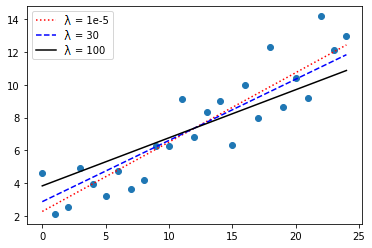
\includegraphics[width=0.8\textwidth]{images/ridge_penalty}
    \caption[Choice of the penalty factor in RR]{The effect of the choice of the penalty factor $\lambda$ on the solution of the ridge regression problem. Adapted from \cite{ridge_penalty}}
    \label{fig:ridge_penalty}
\end{figure}

Note that the intercept $\beta_0$ is left out of the penalty term, as penalizing the intercept would make the procedure dependent on the scale of $\mathbf{y}$.

The linear regression problem solved by minimizing the L2-regularized RSS above is called \textbf{ridge regression} problem \cite{ridge, hastie}.
Ridge regression has the following closed form solution
\[
\hat{\bm{\beta}}^\text{ridge} = (X^TX+\lambda I_0)^{-1}X^T\mathbf{y}
\]

As we can observe, a positive constant is added to the diagonal of $X^TX$ before inversion: this makes the resulting matrix non-singular even when $X^TX$ is, thus making the linear regression problem well-conditioned. Notice also that due to the addition of $\lambda I_0$ ridge estimates are not equivariant under scaling of the inputs (as opposed to OLS), and so one normally standardizes the dataset before solving the ridge regression problem.

In many experimental contexts, $X$ is a very large matrix. In such cases, the matrix $X^TX$ and the inverse of $X^TX+\lambda I_0$ are very expensive to compute. For this reason, when $N$ and/or $M$ are particularly large, the ridge regression problem is solved iteratively via SGD (sec. \ref{sec:sgd}).





\subsection{Random forest}
\label{sec:random_forest}
\textbf{Random forest} \cite{random_forest, hastie} is an ensemble learning method for classification and regression tasks, which performs prediction through majority voting (classification) or averaging (regression) the predictions of an ensemble of decision trees. In this section, we will discuss only random forest regression.

A regression tree is a simple regression model that predicts the response variable $y$ associated to a sample $\mathbf{x}$ by traveling from its \textit{root node} to one of its \textit{leaves}. At each node on the root-to-leaf path, the successor node is chosen on the basis of a splitting of the input space. Usually, the splitting is a binary "test" on one of the features of $\mathbf{x}$. In this way, a decision tree tesselates the input space with non-overlapping hyper-rectangles ("boxes") in which a certain number ($\geq1$) of training samples are located. A prediction is made by averaging the ground-truth labels of the training samples located in the input space box associated to the leaf reached. An example is shown in fig. \ref{fig:regr_tree}.

\begin{figure}[hbt!]
    \centering
    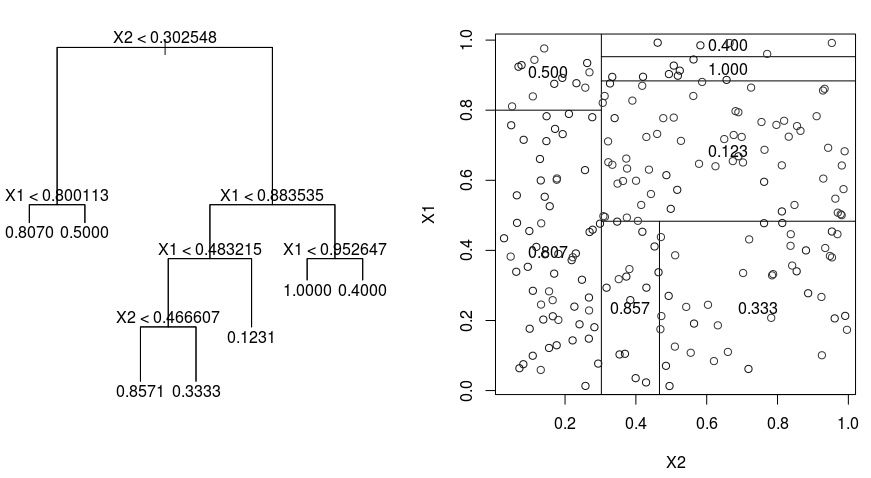
\includegraphics[width=\textwidth]{images/regr_tree}
    \caption[A regression tree and the induced tesselation of the input space]{A regression tree trained on a 2D dataset (left), and the induced tesselation of the input space (right). Taken from \cite{regr_tree_img}}
    \label{fig:regr_tree}
\end{figure}

Although many different regression tree learning algorithms exist, most of them follow the same approach, known as recursive binary splitting. This approach is:
\begin{itemize}
    \item top-down: the tree is built recursively starting from the root and going down to the leaves
    \item greedy: at each recursive step the local best split is performed, rather than a locally suboptimal one which might lead to the globally optimal tree
\end{itemize}

Different learning algorithms use different metrics for defining the "best" predictor on which to split the training samples, and the associated test to perform on it. These metrics generally measure the "homogeneity" of the target variable within a set of samples. One of the most commonly used is variance reduction \cite{variance_reduction}. The variance reduction of a node is defined as the total reduction of the variance of the target variable $y$ due to the split at this node; the predictor on which to split is the one which would cause the largest variance reduction.

This training process would continue to expand nodes by minimizing the chosen metric, until all leaves are homogeneous (i.e. all the training samples in the input space box associated to each leaf have the same response variable). Clearly, this may lead to overfitting the training data. To prevent it, we may decide to build the tree until a stopping criterion is reached: for example, we could fix the maximum depth of the tree as a hyperparameter of the learning algorithm (\texttt{max\_depth} in scikit-learn \cite{sklearn_random_forest}).

\smallskip

Regression trees are simple, highly interpretable and can be displayed graphically. However, they typically can't compete with other well-known regression approaches in terms of prediction performances. To reduce variance, prevent overfitting and hence increase performances, we may train a random forest, an ensemble learning technique that consists in growing multiple regression trees and then combining them to produce a prediction based on averaging the predictions given by each tree. It is based on two statistical techniques:
\begin{itemize}
    \item Bagging (bootstrap aggregating) \cite{bagging}: train an ensemble of $B$ models on $B$ different training sets, each obtained by randomly sampling $N$ instances with replacement from the original training set of $N$ samples; used to reduce the variance of a learning algorithm
    \item Feature bagging (random subspace method) \cite{feature_bagging}: at each split, the features on which to split are selected within a random subset of only $M'<M$ of the total set of $M$ predictors (a typical choice is $M'=\sqrt{M}$); used to reduce the correlation between regression trees in an ensemble
\end{itemize}

Combining many trees usually results in dramatic improvements in performances, at the expense of some loss of interpretability. An example of a random forest is reported in fig. \ref{fig:random_forest}.

\begin{figure}[hbt!]
    \centering
    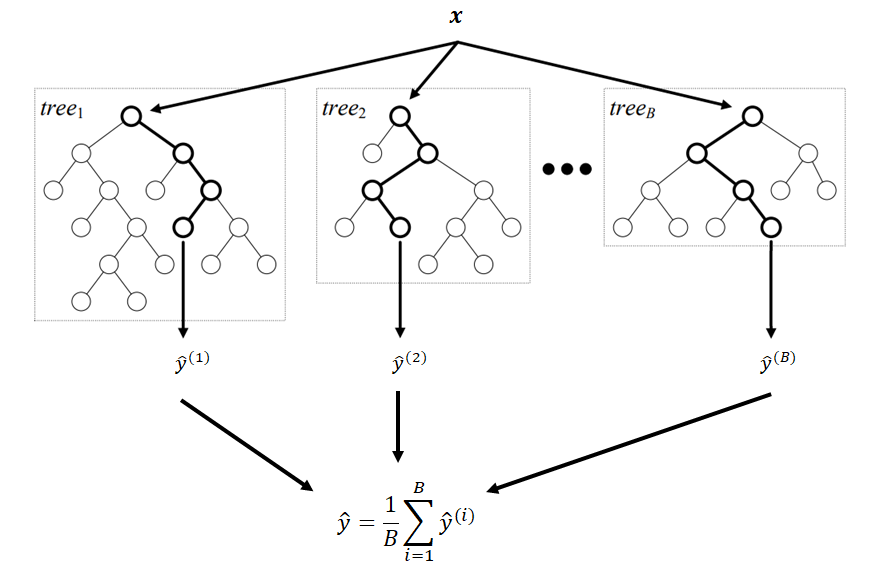
\includegraphics[width=\textwidth]{images/random_forest}
    \caption[A RF with $B$ regression trees]{A random forest regression model with $B$ regression trees. Adapted from \cite{random_forest_img}}
    \label{fig:random_forest}
\end{figure}





\subsection{Feed-forward neural network}
\label{sec:neural_network}
A \textbf{feed-forward neural network} (or simply neural network) is a non-linear model which can be used for regression tasks. The central idea is to extract linear combinations of the input variables as derived features, and then model the target as a nonlinear function of these features.

The "building block" of a neural network is the neuron, shown in fig. \ref{fig:neuron}

\begin{figure}
    \centering
    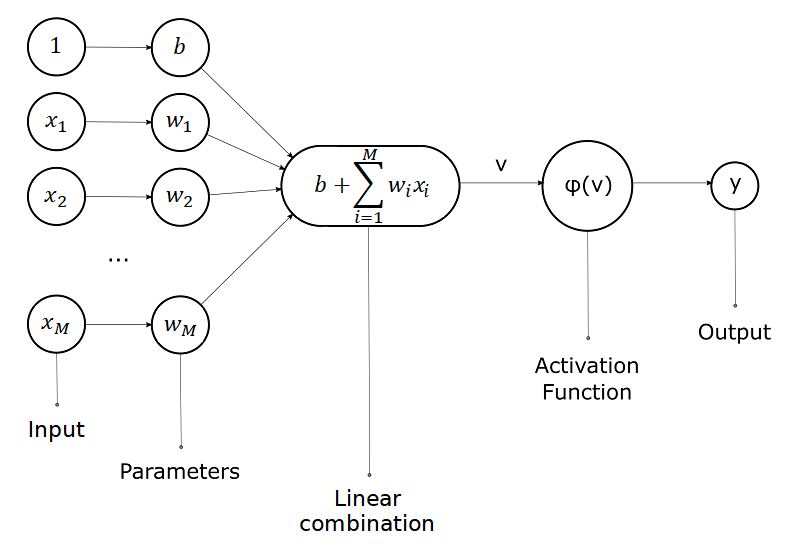
\includegraphics[width=0.9\textwidth]{images/neuron}
    \caption[A neuron in a NN]{A neuron in a neural network.}
    \label{fig:neuron}
\end{figure}

Inside a neuron, the linear combination of an input vector $\mathbf{x}$ with weights $w_1,\dots,w_M$ and bias $b$ is computed, which is then used as the argument of a so-called activation function. The activation function is a non-linear function used to make the neuron a non-linear model.

Neural networks are modeled as collections of neurons that are connected in a directed acyclic graph (DAG). In other words, the outputs of some neurons can become inputs to other neurons. The neurons of a neural network are organized into distinct layers of neurons, called fully-connected (FC) layers: each neuron of layer $i$ is connected to all the neurons of layer $i+1$. The FC layers between the input layer and the output layer are called hidden layers. The neurons of an output layer typically have the identity function as activation function. An example of a neural network architecture is depicted in fig. \ref{fig:neural_network}.

\begin{figure}[hbt!]
    \centering
    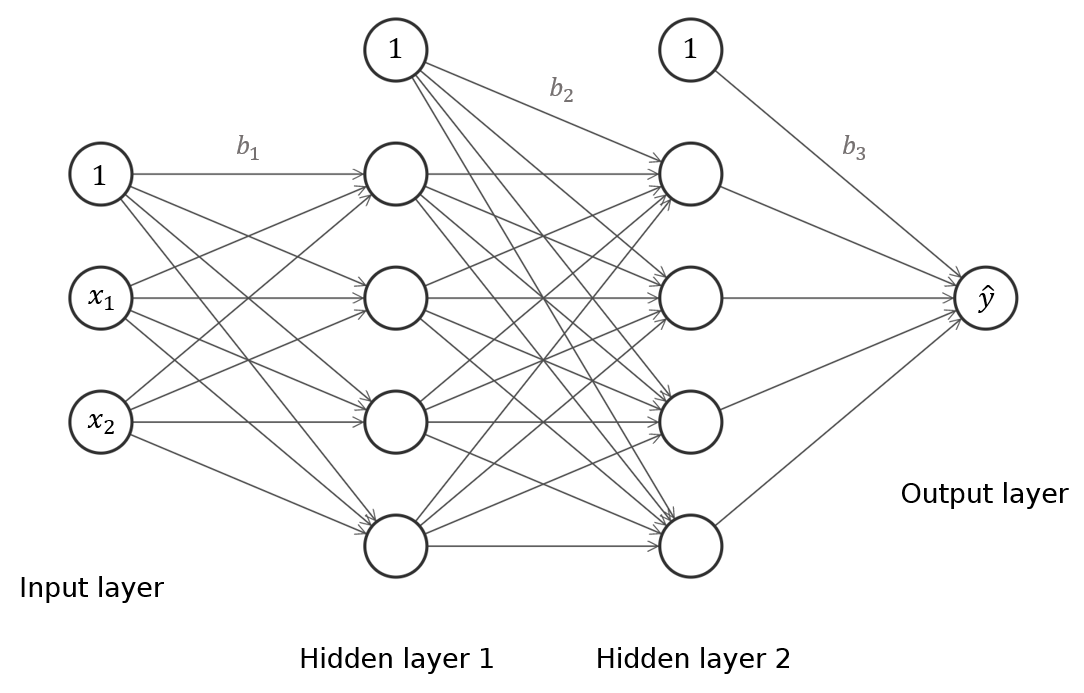
\includegraphics[width=\textwidth]{images/neural_network}
    \caption[A NN with 2 hidden layers]{A feed-forward neural network with a 2D input and 2 hidden layers with 4 neurons each.}
    \label{fig:neural_network}
\end{figure}

Each hidden layer extracts multiple hidden features from the input. Use of multiple hidden layers allows construction of hierarchical features at different levels of resolution \cite{hastie}.

The number of layers $L$ in a neural network, the number of neurons $N_1,\dots,N_L$ in each layer and the activation function $\phi$ for each neuron are hyperparameters to be optimized via e.g. grid search cross-validation (sec. \ref{sec:cv}), random search or simply by trial and error. The complexity of a neural network is measured by the number of its free parameters (weights and biases), which in turn depends by $L$ and $N_1,\dots,N_L$.

Due to neurons being non-linear models (thanks to the non-linear activation function), the neural network too is a non-linear model.
More complex neural networks are more expensive to train and to perform predictions with, but they have a higher representational power (i.e. they can learn functions which are more non-linear). On the other hand, neural networks which are too complex may overfit the training set, but this issue can be solved with proper regularization of the weights (as discussed in the next section).

\subsubsection{Training}
\label{sec:training_nn}
Training a neural network means estimating its weights and biases (collectively called "learnable parameters", $\bm{\theta}$) in such a way that the predicted values for the target variable associated to the training samples $\mathbf{x}_{1},\dots,\mathbf{x}_{N}$ are close to the ground-truth targets $y_1,\dots,y_N$. More specifically, we seek to find $\mathbf{w}^{(1)} \in \mathbb{R}^{N_1},\dots,\mathbf{w}^{(L)} \in \mathbb{R}^{N_L}$ and $\mathbf{b} \in \mathbb{R}^L$ such that the L2-regularized mean squared error (MSE) cost function
\begin{equation}
\text{MSE}_\text{L2}(\bm{\theta};X,\lambda) = \frac{1}{N} \sum_{i=1}^N(y_i-f(\mathbf{x}_{i};\bm{\theta}))^2 + \frac{1}{2}\lambda \sum_{w\in \bm{\theta} \setminus \mathbf{b}} w^2
\end{equation}
is minimized. The penalty factor $\lambda$ (also called \textit{weight decay} in the context of neural networks) measures how strongly large weights\footnote{Regularization is not applied to biases, for the same reason discussed in sec. \ref{sec:ridge} for ridge regression.} are to be penalized. Choosing $\lambda$ carefully is crucial to prevent overfitting the training set, as evident in fig. \ref{fig:lambda_nn}.

\begin{figure}[hbt!]
    \centering
    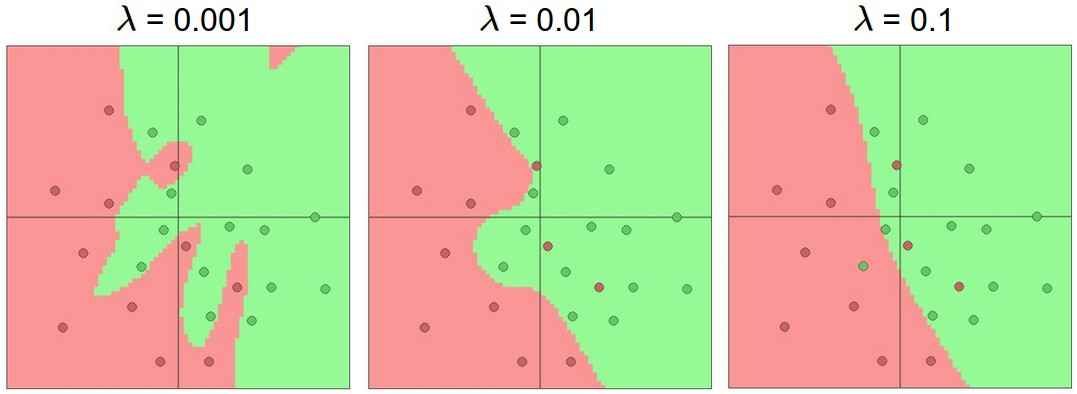
\includegraphics[width=0.9\textwidth]{images/lambda_nn}
    \caption[Decision boundaries of a NN for classification]{Decision boundaries of a neural network trained on a 2D dataset for a classification task, for varying values of $\lambda$. Taken from \cite{cs231n:nn1}}
    \label{fig:lambda_nn}
\end{figure}

As $f$ is a highly non-linear function in general, a closed form solution for the neural network learning problem is too impractical; rather, the problem is usually solved iteratively via SGD (sec. \ref{sec:sgd}).

SGD requires the gradient of the cost function $\mathcal{L}=\text{MSE}_{L2}$ with respect to each learnable parameter ($\nabla_{\bm{\theta}} \mathcal{L}$) to perform an update. Due to the particular topology of a feed-forward neural network, there exists a very efficient way of computing $\nabla_{\bm{\theta}} \mathcal{L}$ analytically, called \textbf{backpropagation} \cite{backprop}. Backpropagation computes each $\partial \mathcal{L}/\partial \theta$ through recursive application of the chain rule; its name suggests the idea that the prediction error is "propagated back" to the parameters "causing" it, and each $\partial \mathcal{L}/\partial \theta$ quantifies how much $\theta$ contributes to the error, thus how steeply we can update the parameter $\theta$ in order to minimize the error.

The depth of the neural network as well as the activation function must be chosen carefully, to avoid the vanishing gradient problem \cite{vanishing_gradient}. In particular, the network should be not too deep, otherwise the gradient of the cost function with respect to early layers' parameters would likely get small (because of a long chain of products between many quantities smaller than 1) and they would be updated very slowly (the neural network would not "learn" anymore). Moreover, the activation function should not operate in regions where it has a derivative approaching zero, as this would effectively kill the gradients of the parameters preceding that activation function. A very popular choice for the activation function is the Rectified Linear Unit (ReLU) \cite{relu}, $\phi(x) = \max(0,x)$, represented in fig. \ref{fig:relu}. ReLU has the advantage of being scale-invariant $(\max(0,ax)=a(\max(0,x))$, cheap to compute (only a comparison between $0$ and $x$ is needed) and non-saturating for $x>0$, which mitigates the vanishing gradient problem. On top of that, ReLU seems to work very well in practice \cite{relu_and_initialization}.

\begin{figure}[hbt!]
    \centering
    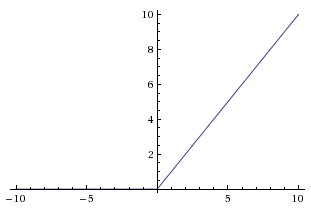
\includegraphics[width=0.6\textwidth]{images/relu}
    \caption[ReLU function]{ReLU function. Taken from \cite{cs231n:nn1}}
    \label{fig:relu}
\end{figure}

When training a neural network, it is common sense to standardize the data, as the scale of the training data has a relevant effect on the scale of the learned parameters and thus on the quality of the final solution. Having input variables scaled to zero mean and unit standard deviation implies that each feature will be deemed equally relevant in the learning process, and it can be shown that this improves the rate of convergence of training a neural network \cite{nn_standardization}.

Lastly, also the particular initialization of the parameters affects the rate of convergence of training. In particular, the cost function $\text{MSE}_\text{L2}$ is nonconvex and typically exhibits many local minima; as a result the estimates of the parameters are very sensible to their initialization. The recommended heuristic for initializing weights when using ReLU activation functions is Kaiming-He initialization \cite{relu_and_initialization}, which consists in drawing the initial value of each weight $w$ randomly according to a normal distribution
\[
w \sim \mathcal{N}\left(0,\frac{2}{n}\right)
\]
where $n$ is the number of inputs to a specific neuron (i.e. $n = |\mathbf{w_{l-1}}|$ where $l$ is the layer in which the neuron is located); biases, instead, are initialized to 0.
It can be proved that Kaiming-He initialization ensures that all neurons in the network initially have approximately the same output distribution with variance 1 and empirically improves the rate of convergence of the training process.





\section{Performance metrics for regression}
\label{sec:metrics}
To evaluate the performances of a regression model $f$, many different performance metrics can be used \cite{metrics}. These metrics generally measure how good (or bad) $f$ is at estimating the ground-truth target $y$ of a sample, i.e. how close (far) are the predictions $f(\mathbf{x}_{i};\bm{\theta}) = \hat{y}_i$ from $y_i$.
\begin{itemize}
    \item Mean squared error (MSE)
    \[
    \text{MSE} = \frac{1}{N} \sum_{i=1}^N (\hat{y}_i-y_i)^2
    \]
    It gives information on the prediction error that is committed on average. However, due to squaring, this metric does not have the same unit of measurement as the quantity that is being predicted; therefore, other metrics such as the RMSE or the MAE are usually preferred.
    \item Sum of squared errors (SSE)
    \[
    \text{SSE} = \sum_{i=1}^N (\hat{y}_i-y_i)^2
    \]
    Similar to the MSE but with a sum instead of an average operation.
    \item Root mean squared error (RMSE)
    \[
    \text{RMSE} = \sqrt{\frac{1}{N} \sum_{i=1}^N (\hat{y}_i-y_i)^2}
    \]
    It is similar to the MSE, but has the same unit of measurement as the target variable; however, it has no straightforward interpretation.
    \item Mean absolute error (MAE)
    \[
    \text{MAE} = \frac{1}{N} \sum_{i=1}^N |\hat{y}_i-y_i|
    \]
    It measures the average absolute difference between the predicted and real target values.
    \item Coefficient of determination ($R^2$)
    \[
    R^2 = 1 - \frac{\sum_{i=1}^N (y_i-\hat{y_i})^2}{\sum_{i=1}^N (y_i-\overline{y})^2}
    \]
    where $\overline{y}=\frac{1}{N}\sum_{i=1}^N y_i$.
    It provides a measure of how well the predictions $\hat{y}_i$ approximate the true values $y_i$. An $R^2$ of 1 indicates perfect prediction, whereas a model that always predicts the average value of y disregarding the input features ($f(\mathbf{x}_{i};\bm{\theta})=\overline{y}$) would get an $R^2$ of 0. The $R^2$ can also be negative, because the model can do arbitrarily worse than said constant model, in terms of MSE.
    The $R^2$ is not defined when $\overline{y}=y_1=\dots=y_N$; in this case, we set $R^2=1$ for perfect prediction and $R^2=0$ for imperfect prediction.
\end{itemize}





\section{\textit{K}-fold cross-validation}
\label{sec:cv}
To tune the hyperparameters which characterize a regression procedure\footnote{By "procedure" we refer in general to the whole training pipeline of a regression model, including data cleaning, data preprocessing and feature extraction steps. In fact, also these earlier steps can be characterized by user-defined hyperparameters, which are to be optimized.}, \textbf{(stratified) $K$-fold cross validation} can be used. It consists in randomly splitting the training set into $K$ subsets, called \textit{folds}. One fold is held out as a validation set, while the remaining $K-1$ folds are used for training the model: each prediction pipeline is fitted and trained on the $K-1$ training folds, and tested on the remaining validation fold, on which one or more performance metrics are evaluated (e.g. MSE or MAE). This procedure is repeated $K$ times, in order to use each fold as a validation set; therefore a total of $K$ regression models are trained. The resulting performance metrics are combined (e.g. averaged) over the $K$ rounds to give an estimate of the model's predictive performance on unseen data.

Typically, a grid search over different hyperparameters is performed through cross-validation. The hyperparameter combination achieving the highest cross-validation score is considered the optimal one, and the regression procedure with the optimal hyperparameters is refit on the whole training set, thus obtaining the final regression model. The cross-validation procedure is visually summarized in fig. \ref{fig:cross_validation}.

\begin{figure}[hbt!]
    \centering
    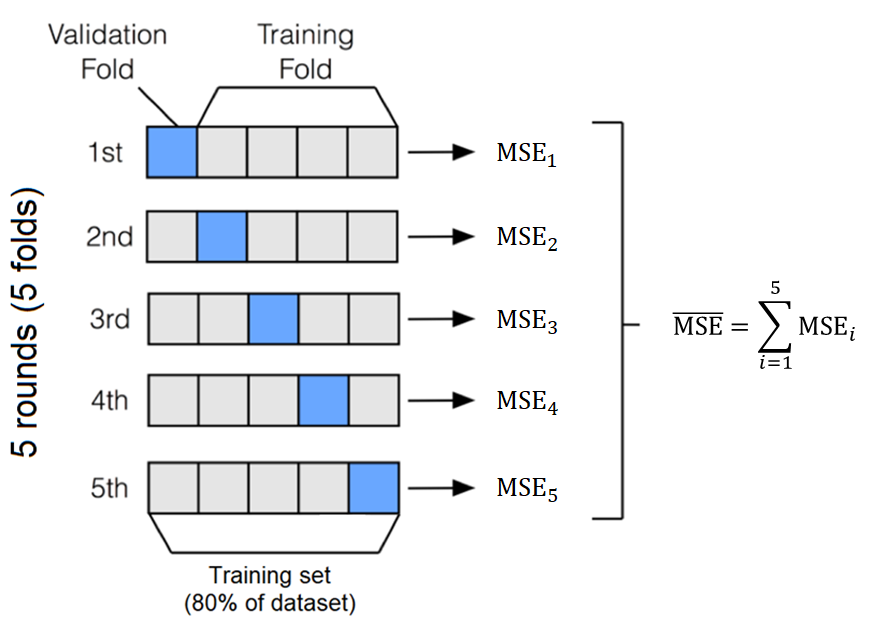
\includegraphics[width=0.9\textwidth]{images/cross_validation}
    \caption[5-fold cross-validation]{5-fold cross-validation procedure adopted in the experiments of this thesis (see sec. \ref{sec:regr_model_training}).}
    \label{fig:cross_validation}
\end{figure}